\documentclass[10pt,a4paper,openany]{book}
\usepackage[utf8]{inputenc}
\usepackage[spanish,es-nodecimaldot]{babel}
\usepackage{amsmath}
\usepackage{amsfonts}
\usepackage{amssymb}
\usepackage{graphicx}
\usepackage{xcolor}
\usepackage{lipsum}
\usepackage{pdfpages}
\usepackage{tocbibind}
\usepackage{setspace}
\usepackage{fancyhdr}
\usepackage{wrapfig,lipsum,booktabs}
\usepackage{float}
\usepackage{subfig}
\usepackage{wrapfig}
\usepackage{multicol}
% \pagestyle{fancy}
% \fancyhf{}
% \lhead[\leftmark]{Nombre Autor}
% \rhead[Nombre Autor]{\rightmark}
% \lfoot[]{página \thepage}
% \rfoot[página \thepage]{}

% Contador para subsubsection, para que aparezca en la tabla de contenidos
\setcounter{tocdepth}{3}
\setcounter{secnumdepth}{3}
% -------------- quitar el ":" de las figuras"
\makeatletter
\long\def\@makecaption#1#2{
\vskip\abovecaptionskip
\sbox\@tempboxa{#1. #2}
\ifdim \wd\@tempboxa >\hsize
#1. #2\par
\else
\global \@minipagefalse
\hb@xt@\hsize{\hfil\box\@tempboxa\hfil}
\fi
\vskip\belowcaptionskip}
\makeatother
% ---------------------------------------


\usepackage[left=2.54cm,right=2.54cm,top=2.54cm, bottom=2.54cm]{geometry}
\author{Jiménez Ramos Miguel}
\title{Proyecto}
\begin{document}

 \includepdf{caratula/caratulad.pdf}
 \renewcommand{\thechapter}{\Roman{chapter}}
 \renewcommand*\contentsname{Contenido}


\tableofcontents
\listoffigures

\chapter*{} % para comenzar la numeracion de paginas en numeros romanos
\begin{flushright}
\textit{\Large Si he visto más lejos que otros,\\ es porque me he subido en hombros de gigantes.}
\vspace{1cm}

\text{ISAAC NEWTON}
\end{flushright}
\chapter{Flujo laminar}
\section{Breve resumen}
\onehalfspacing
La medicina hoy en día juega un papel fundamental en nuestras vidas, está ahí para mejorar nuestra calidad de vida, y de ese modo tener una vida plena, sin males ni rarezas.
Lo espléndido de la medicina es que se relaciona inherentemente a las matemáticas, dando resultados sumamente magníficos e interesantes, los cuales vale la pena estudiar a profundidad y con suma dedicación.
Por ejemplo, el flujo sanguíneo es una de tantas temáticas que posee bastante material cautivador para un proyecto de aplicación, dentro de este tema podemos encontrar principios y leyes bastante fuertes, una de ellas es la \textbf{ley de Poiseuille}, la cual nos explica que dado un flujo de sangre que circula por un vaso sanguíneo con un flujo $F$, dicho flujo es proporcional a la cuarta potencia del radio R del vaso sanguíneo. 
\begin{align}
    F=kR^{4} \label{first}
\end{align}
En el transcurso del presente texto se profundizará con detalle el razonamiento detrás de las expresiones matemáticas que describen de manera sorprendente hechos que  son inherentes a un ser vivo. Como complemento a la información presentada en el texto, se tendrá en cuenta hacer uso de recursos visuales, tales como gráficas, dibujos y demás, esto con la finalidad que el lector pueda comprender todas las ideas fundamentales que se requieren para asimilar la información del escrito.\\
\section{Análisis}
Se aplicará primeramente un análisis a la función de interés, con el propósito de proveer un panorama mas detallado para el lector. \\ \\
Los criterios para el análisis serán los siguientes:\\
\begin{itemize}
    \item Dominio de la función.
    \item Dominio de la función en el contexto de aplicación.
    \item Primera derivada (significado).
    \item Segunda derivada (significado).
    \item Mínimos y máximos (Globales y locales).
    \item Graficar primera y segunda derivada haciendo uso de software.
    \item Denotar las características matemáticas más importantes (límites, continuidad, etc.)
\end{itemize}
Resultaría pertinente mencionar las funciones que son objeto de estudio en materia de medicina; sin embargo solo se mencionará aquella que sea, por así decirlo, especial, esto se refiere a que nos proporcione información impactante, de la cual podamos concluir afirmaciones fuertes. En particular, hablaremos de \textbf{la ley del flujo laminar}.

\vspace{0.5cm}\begin{figure}[h]
    \centering
    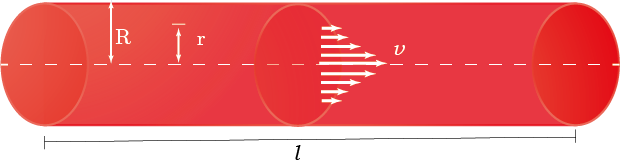
\includegraphics[scale=2.1]{imagenes/a.png}{}
    \caption{Flujo laminar en una arteria.}
    \label{fig:my_label}
\end{figure}
% First poise ecuation
\begin{align}
    v(r)=\frac{P}{4\eta l}(R^{2}-r^{2}) , \label{Poise} 
\end{align}

\vspace{0.5cm}
donde cada elemento de la expresión significa lo siguiente:
\begin{itemize}
    \item P es la diferencia de presiones entre los extremos de la arteria.
    \item $\eta$ es el coeficiente de viscosidad de la sangre.
    \item $l$ es la longitud de la arteria.
    \item $R$ denota la longitud del radio de la arteria.
    \item Podemos considerar el flujo sanguíneo como un cilindro coaxial a la arteria, la cual es un cilindro. Entonces, nombremos el radio de este cilindro coaxial como $r$. 
    \item Además, $P,\eta,l,R>0$ y $R\geq r\geq0.$
\end{itemize}
Una vez mencionado todo lo anterior sería oportuno adentrarnos en el análisis del que se hace mención.
\subsection{Dominio}
La función \ref{Poise} es interesante, exige comprender precisamente algunas restricciones que por muy evidentes que sean, eventualmente, pasan desapercibidas. Demos un vistazo a la figura \ref{fig:my_label}, obsérvese que $r$ no puede ser mayor que $R$, en caso contrario caeríamos en un absurdo, ya que no tendría sentido considerar un cilindro coaxial  (referente al flujo laminar) el cual sea mayor que la propia arteria, tan solo imagínelo basándose en la figura \ref{fig:my_label}. Otra restricción es que $R \hspace{0.09cm} y \hspace{0.09cm}l\hspace{0.1cm}$ tienen que ser \textbf{estrictamente mayores a cero}, ya que no existen longitudes negativas, además por nuestros propósitos se pide que no sean cero. Posiblemente en algún universo paralelo (si es que existe) usted y yo estemos tan lejos o tan cerca negativamente, no obstante, en este no.\\ \\
Lo anterior nos puede sugerir el dominio para la función \ref{Poise}, véase a continuación:
\begin{align}
    Dom(v)=r\in \left[0,R\right]. \label{dom1}
\end{align}
Bien, cabe destacar que, en efecto, este es el dominio en el \textbf{contexto de aplicación}, aunque también falta considerar el dominio de la función en un contexto puramente matemático. Un posible dominio a considerar sería:
\begin{align}
    Dom(v)=\left\lbrace
    r/r\in \mathbb{R^+}
    \right\rbrace, \label{dom2}
\end{align}
podemos considerar otros dominios tales que $v(r)$ pueda ser sea negativa, o bien, positiva. Un dominio donde la función $v$ tome ambos valores sería el siguiente:
\begin{align}
    Dom(v)=\left\lbrace
    r/r\in \mathbb{R}
    \right\rbrace. \label{dom3}
\end{align}
\subsection{Primera y segunda derivada}
Es una buena practica observar en qué categoría se encuentran las funciones que vamos conociendo a lo largo del tiempo, esto nos puede ayudar a darnos una idea sobre el comportamiento de las mismas, y, de ese modo, se facilite su respectivo análisis. En nuestro caso particular, puede apreciarse que estamos tratando con una función polinómica (\ref{Poise}), lo cual tiene implicaciones importantes de nuestro interés, como bien podría ser su continuidad y diferenciabilidad. Singularmente, esta función cumple que es continua en todo su dominio (ya sea \ref{dom1}, \ref{dom2} o bien \ref{dom3}) y derivable en todo su dominio (\ref{dom3}). Esto nos motiva a obtener la primera y la segunda derivada, es por ello que a continuación se apreciará el proceso de diferenciación de esta función sobre el dominio \ref{dom3} (más adelante se explicará por qué no sobre \ref{dom1}).
\begin{align}
    Sea \hspace{0.5cm} v(r)&=\frac{P}{4\eta l}(R^{2}-r^{2})\\
    \frac{dv}{dr}&=\frac{P}{4\eta l}\left[\frac{d}{dr}\left(R^{2}-r^{2}\right)\right]\\
    &=\frac{P}{4\eta l}\left[\frac{d}{dr}R^{2}-\frac{d}{dr}r^{2}\right]\\
    &=\frac{P}{4\eta l}\left[0-\frac{d}{dr}r^{2}\right]\\
    &=\frac{P}{4\eta l}\left[-2r\right]\\
    &=-\frac{Pr}{2\eta l}. \hspace{0.1cm}\label{derivative_one} \text{ $(Observar\ que \ es \ lineal \ en\ v).$ }
\end{align}

 Obteniéndose de este modo, la razón de cambio de la velocidad del flujo laminar, también llamado gradiente de velocidad. Es interesante observar que esta nueva función es negativa, una primera pregunta sería: ¿Qué nos quiere decir que el gradiente de velocidad sea negativo, y qué implicaciones tiene? Pensemos un momento en la figura \ref{fig:my_label}, note que la velocidad del flujo laminar ``$v$'' decrece conforme se aleja del eje principal, lo que nos hace pensar que dado un radio $r$, el gradiente de velocidad con unidades $(m/s)/m$, disminuye a una velocidad determinada por cada metro que se aleja del eje principal.\\ \\
 Posiblemente el lector se estará preguntando sobre cómo obtener la velocidad del flujo laminar en el eje principal, por supuesto, esta pregunta aparece inmediatamente por lo mencionado anteriormente que es referente al hecho de que la velocidad decrece lejos del eje principal. Podemos expresar
 \textbf{la velocidad del flujo laminar} en el eje principal ``$v_{p}$'' como el siguiente límite de la función $v$ sobre el dominio de aplicación (\ref{dom1}).
 
 \begin{align*}
     v_{p}=\lim\limits_{r \to 0^+}\left[\frac{P}{4\eta l}\left(R^2-r^2\right)\right].\\
 \end{align*}
 
 Para un dominio como \ref{dom3} puede considerar simplemente el límite de la función $v$, siempre y cuando el límite exista. Note que consideramos el límite por derecha estrictamente, esto por el dominio de aplicación. Puede ver que esto hace perfecto sentido, además, es bastante intuitivo de ver si nos basamos en la figura \ref{fig:my_label}; a medida que el radio se hace suficientemente pequeño nos acercamos más a la velocidad ilustrada en el eje principal (la flecha más larga). Desarrollaremos el límite, véase a continuación.
 
  \begin{align*}
     &\frac{P}{4\eta l}\left[\lim\limits_{r \to 0^+}\left(R^2-r^2\right)\right]\\
     &=\frac{P}{4\eta l}\left[\lim\limits_{r \to 0^+}R^2-\lim\limits_{r \to 0^+}r^2\right]\\
     &=\frac{P}{4\eta l}\left[R^2-0\right] \hspace{1cm} \hspace{1cm} \text{por $r^2$ continua en $\mathbb{R}$}\\
     &=\frac{PR^2}{4\eta l}.\\
 \end{align*}
 Para que esto resulte más intuitivo podemos proponer unos valores para las constantes de nuestra función que estamos analizando. Consideraremos valores estándar para los parámetros de la función \ref{Poise}, por supuesto, apoyándonos sobre los datos de una artería promedio de un ser humano, basándonos en un estudio realizado en la india sobre algunos parámetros de la arteria cubital en adultos al sur de rajastán\footnote{Rajastán es un estado del norte de la india que limita con pakistán.}(Beniwal et al., 2014), por ejemplo. Es importante destacar que trabajaremos sobre el sistema de unidades MKS\footnote{El sistema MKS de unidades expresa las medidas utilizando como unidades fundamentales metro, kilogramo y segundo.}(únicamente en los cálculos aritméticos), para que no haya confusiones respecto al manejo de unidades.\\
 
 Sea $\eta=0.003\left[\frac{Ns}{m^2}\right]$, $l=0.002\left[m\right]$, $P=3.9\left[\frac{N}{m^2}\right]$ y $R=8\cdot10^{-5}\left[m\right]$, dados estos valores, sustituyendo tenemos lo siguiente:
 
\begin{align}
    v(r)=\frac{3.9\left[\frac{N}{m^2}\right]}{4\left(0.003\left[\frac{Ns}{m^2}\right]\right)\cdot\left(0.002\left[m\right]\right)}\left[\left(8\cdot10^{-5}\left[m\right]\right)^{2}-r^{2}\right]. \label{poiseUnits}
\end{align}
 \\
 Recordemos que $r$ es una variable independiente, de la cual, la función $v$ depende. Ahora bien, calcular la velocidad en el eje principal no debería ser ningún problema, debido a que ya lo hicimos, y abordando a este caso en particular, sería como se puede apreciar en la siguiente expresión.
 
  \begin{align*}
     v_{p}=\lim\limits_{r \to 0^+}\left[\frac{P}{4\eta l}\left(R^2-r^2\right)\right]=\frac{PR^2}{4\eta l}.\\
 \end{align*}
 Particularmente tenemos:
\begin{align*}
    v_{p}=&\frac{3.9\left[\frac{N}{m^2}\right]\cdot\left(8\cdot10^{-5}\left[m\right]\right)^2}{4\left(0.003\left[\frac{Ns}{m^2}\right]\right) 
    \left(0.002\left[m\right]\right)}\\ \\
    v_{p}=&1.04\cdot10^{-3}\left[\frac{m}{s}\right].\\
 \end{align*}
 Algo interesante de observar es que además de ser la velocidad en el eje principal, se puede afirmar que es la velocidad máxima del flujo laminar, en esta localidad la fricción respecto a las paredes de la arteria de radio $R$ es considerablemente pequeña, lo que sugiere que sea la mayor velocidad que puede alcanzar dicho fluido.
 \begin{figure}[H]
    \centering
    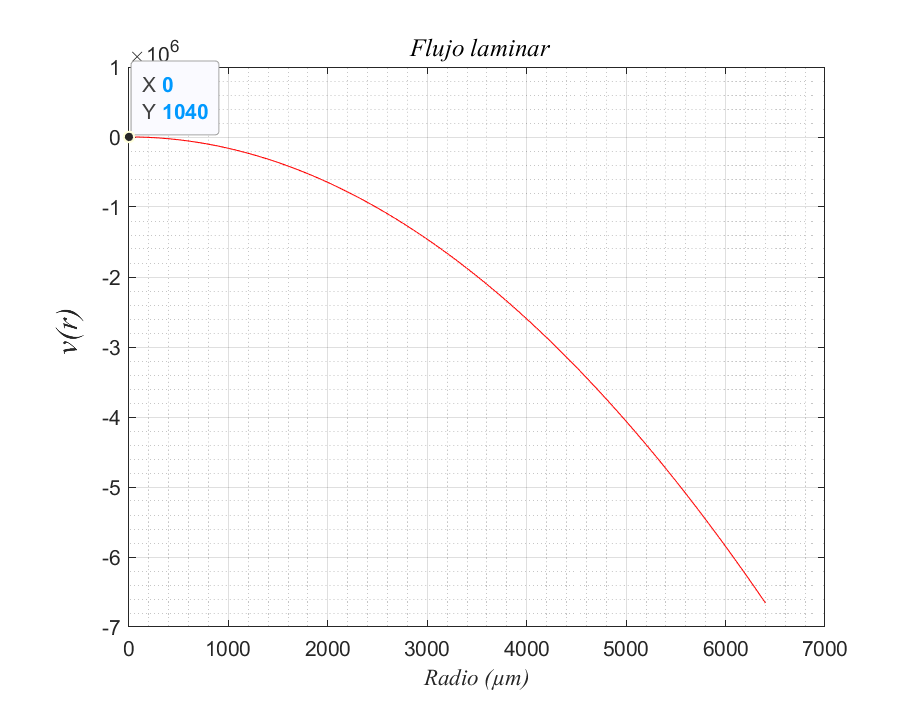
\includegraphics[scale=0.70]{capitulos/graficas/pps.eps}\caption{Velocidad del flujo laminar (Radio $r \ en \ \mu m\ \& \ v(r) \ en\ \mu m/s$).}
    \label{fig:graphic_poise}
\end{figure}
Aclaremos un par de cosas; por motivos prácticos al graficar esta función, resulta tentador cambiar las unidades de la velocidad y distancia por $\frac{\mu m}{s}$ y $\mu$m, cambiar de unidades no debería ser ningún problema para el lector. Por otro lado, para sostener la  afirmación sobre la existencia de este máximo debemos verificar que, en efecto, esta función tiene un \textbf{máximo}. Para esto debemos corroborar unas cuantas cosas.\\
\subsection{Valor máximo}
\subsubsection{Criterio de primera y segunda derivada}

\fbox{\fbox{\parbox{5.5in}{\centering
        \vspace{0.2cm} \textbf{Lema}\\ \vspace{0.2cm} $Si \ f^{'}(x)>0 \ para \ toda \ x\ de \ un \ intervalo\implies$ \hspace{0.01cm} $f\ es\ creciente \ en \ el \ intervalo.$\\
        $Si \ f^{'}(x)<0 \ para \ toda \ x\ de \ un \ intervalo\implies$ \hspace{0.01cm} $f\ es\ decreciente \ en \ el \ intervalo.$\\
        
        \vspace{0.2cm}
        }}}
   \vspace{0.5cm}

Notemos que $v^{'}(r)<0\ (ve\Acute{a}se\ \ref{derivative_one}), \ \ \forall r\in \left[0,R\right]$, por lo tanto la función $v$ es decreciente en todo su dominio. Pero... ¿Qué nos hace pensar esto? Como se menciona, nuestro dominio de aplicación es: 
$$dom(v)=r\in\left[0,R\right].$$ Lo que nos lleva a preguntarnos ¿Será que esto sugiere que la función $v$ tenga un máximo? Es bastante intuitivo ver que efectivamente existe un máximo (figura \ref{fig:graphic_poise}), basta con el hecho de que sea decreciente para darnos cuenta sobre la existencia de este valor máximo en nuestro dominio de aplicación (\ref{dom1}), notemos que no es posible aplicar el criterio de la primera y segunda derivada para determinar máximos de esta función, esto ya que por la naturaleza del dominio no nos permite, obsérvese que al momento de derivar la función las derivadas laterales no son iguales. Sin embargo el criterio de primera y segunda derivada son estrictamente válidos en el dominio \ref{dom3}, es por ello que aclararemos que para este análisis de punto máximo consideraremos el dominio \ref{dom3} en vez del dominio de aplicación. Véase que:

\begin{align*}
    \frac{dv}{dr}=-\frac{Pr}{2\eta l}.
\end{align*}
Haciendo $\frac{dv}{dr}$ igual a cero
\begin{align*}
    -\frac{Pr}{2\eta l}=0,
\end{align*}
luego buscamos una $r$ que satisfaga la ecuación anterior
\begin{align*}
    -Pr&=0\cdot(2\eta l)\\
    r&=-\frac{0}{P} \text{\ ($P\neq$ 0)}\\
    r&=0.
\end{align*}
Nuestro punto singular es $r=0$; ya que lo encontramos, hay que hacer notar un par de cosas, si evaluamos \ref{Poise} en r=0, no salimos del dominio de aplicación y por tanto podemos pensar en lo siguiente:
\begin{align*}
    v(0)&=\frac{P}{4\eta l}(R^{2}-0^{2})\\
    v(0)&=\frac{PR^2}{4 \eta l}
\end{align*}
Particularmente podemos ver que
\begin{align*}
    v(0)&=\frac{3.9\left[\frac{N}{m^2}\right]}{4\left(0.003\left[\frac{Ns}{m^2}\right]\right)\cdot\left(0.002\left[m\right]\right)}\left[\left(8\cdot10^{-5}\left[m\right]\right)^{2}-0^{2}\right]\\
    v(0)&=1.04\cdot10^{-3} \left[\frac{m}{s}\right] \text{ó } 1040\left[\frac{\mu m}{s}\right].
\end{align*}
Queremos verificar que el punto crítico $P(0,1040)$ se trata de un máximo, por ello ocuparemos el criterio de segunda derivada.\\ \\

\fbox{\centering\fbox{\parbox{5.5in}{\centering
        \vspace{0.2cm} \textbf{Teorema}\\ \vspace{0.2cm}
        $Sea\ f\  una\  funci\Acute{o}n\ definida\ en\ alg\Acute{u}n\ intervalo, donde$ \ ``a'' \ $pertene \ a \ dicho \ intervalo $,  \ $si\ f^{'}(a)=0 \ y $ $f^{''}(a)<0 \implies f\ tiene\ m\Acute{a}ximo\ local\ en \ a.$
        \vspace{0.2cm}
        }}}
   \vspace{0.5cm}
\begin{align}
    \frac{d^2v}{dr^2}&=-\frac{P}{2\eta l}\left[\frac{d}{dr}r\right]\\
    \therefore \ \frac{d^2v}{dr^2}&=-\frac{P}{2\eta l}. \label{sencond_derivative_speed}
\end{align}
Notemos que la derivada del gradiente de velocidad es constante y negativa (más adelante se explicará su significado), entonces, por el criterio de la segunda derivada se trata de un punto máximo. Con esto verificamos que, en consecuencia, el punto P(0,1040) se trata de un máximo de \ref{Poise}, más aún, se trata de un máximo global ya que verifica que $\exists r_{0}\in[0,R]\ /v(r_{0})>v(r), \ \forall r \in[0,R].$ También sería interesante anexar las gráficas de la primera y segunda derivada, con el fin de observar su comportamiento.
 \begin{figure}[H]
 \hspace{-0.3cm}
    % \subfloat[Razón de cambio del gradiente de velocidad]{
    % 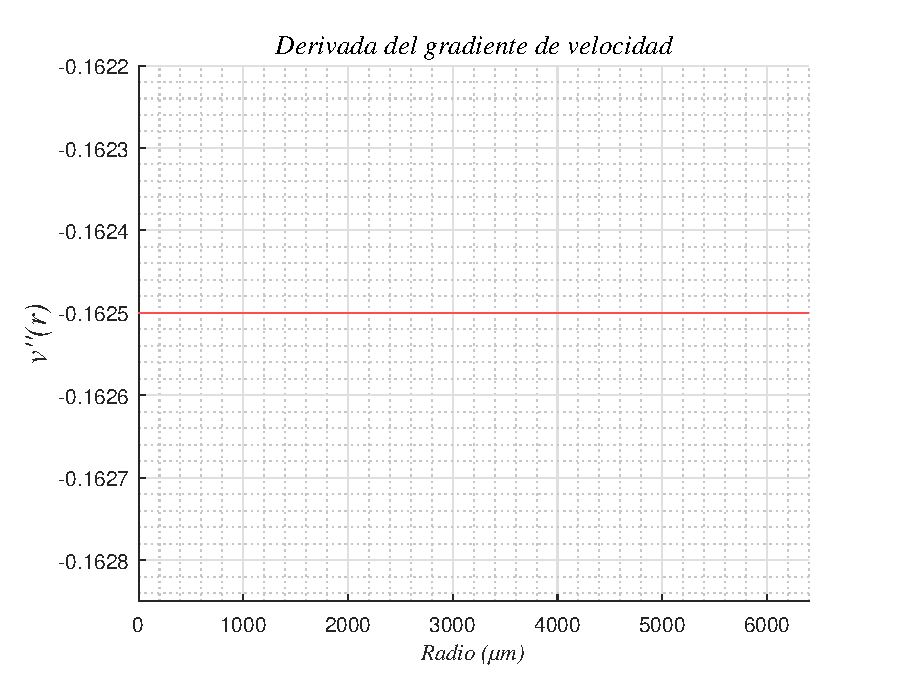
\includegraphics[scale=0.55]{capitulos/graficas/derivadagradiente.eps}
    % \label{fig:graphic_derivada_gradiente_velocidad}}
    \subfloat[Gradiente de velocidad]{
    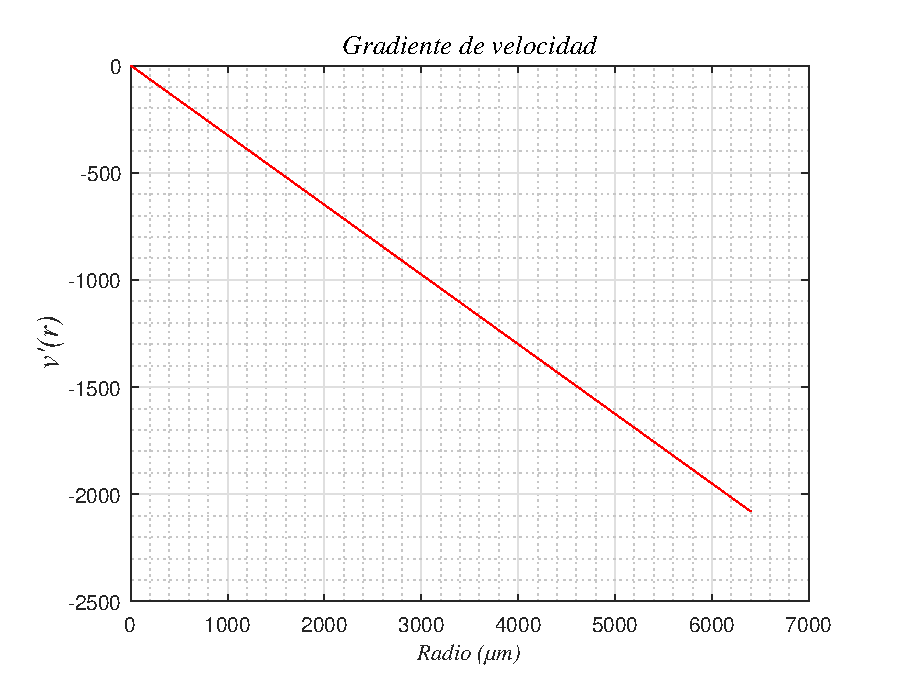
\includegraphics[scale=0.55]{capitulos/graficas/gradientevelocidad.eps}
    \label{fig:graphic_gradiente_velocidads}}
 \subfloat[Derivada del gradiente de velocidad]{
    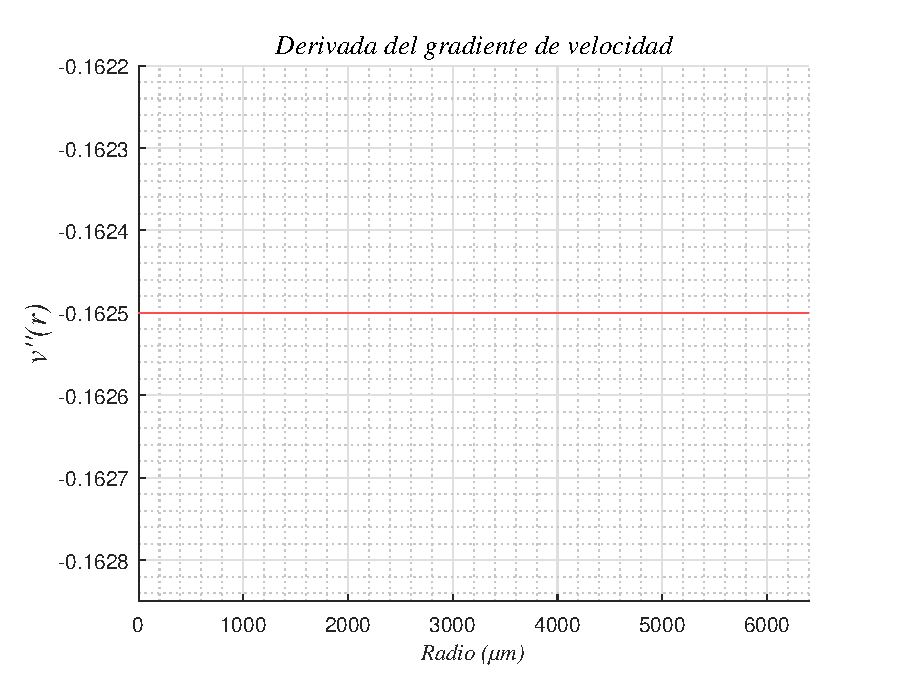
\includegraphics[scale=0.55]{capitulos/graficas/derivadagradiente.eps}
    \label{fig:graphic_Derivada del gradiente de velocidad}}
    \caption{Gráficas de la primera y segunda derivada.}
\end{figure}
Para finalizar con la sección correspondiente al análisis de la primera y la segunda derivada, mencionaremos a qué se refiere la derivada del gradiente de velocidad. Ahora bien, para comprender el significado de la derivada del gradiente de velocidad tendremos que recordar nuevamente el significado del gradiente de velocidad, luego partiremos de ahí para facilitar su comprensión. El gradiente de velocidad (negativo) significa que disminuye la velocidad por cada metro que se aleja del eje principal, las unidades del gradiente de velocidad (MKS) nos dan una respuesta intuitiva $\left(m/s\right)/m$. Para comprender el significado de la derivada del gradiente de velocidad resulta muy similar a la que dimos para el gradiente de velocidad, respectivamente hay que hacer un análisis de las unidades que están involucradas en \ref{sencond_derivative_speed}. Véase a continuación:
\begin{align*}
    \cfrac{\cfrac{N}{m^2}}{\cfrac{Ns}{m^2}\cdot m}=\cfrac{\cfrac{N}{m^2}}{\cfrac{Ns}{m}}=\cfrac{Nm}{Nm^2s}=\frac{Kg\cdot\cfrac{m^2}{s^2}}{Kg\cdot\cfrac{m^3}{s}}=\cfrac{\cfrac{m^2}{s^2}}{\cfrac{m^3}{s}}=\cfrac{\left(\cfrac{s}{m}\right)\cfrac{m^2}{s^2}}{\left(\cfrac{s}{m}\right)\cfrac{m^3}{s}}=\textcolor{red}{\cfrac{\cfrac{m}{s}}{m^2}}
\end{align*}
La derivada del gradiente de velocidad (constante y negativa) significa que disminuye la velocidad constantemente por cada metro cuadrado que se aleja del eje principal, muy similar a lo que mencionamos del gradiente de velocidad, solo con la diferencia que la velocidad disminuye por cada metro cuadrado que se aleja del eje principal.

\subsection{Interpretación sobre teorema de valor medio}
El teorema de valor medio, por sí solo, es uno de tantos teoremas fuertes del cálculo infinitesimal, esto es ya que nos permite deducir otras proposiciones que son consecuencia directa de este teorema, tales proposiciones tienen implicaciones bastante fuertes en las matemáticas; un ejemplo de un teorema fuerte que se puede demostrar con ayuda del teorema de valor medio es el \textbf{teorema de Taylor}, el cual será objeto de estudio en algún otro curso de matemáticas avanzadas, no obstante este teorema se relaciona intrínsecamente con el cálculo infinitesimal, lo cual resulta interesante y bello. Enunciaremos a continuación el teorema de valor medio, pero antes daremos la definición de la tasa de variación media de una función $f$ en $[a,b]$, con el propósito de tener todo en orden y bien definido.
\vspace{0.9cm}
\subsubsection{Tasa de variación media y un teorema fuerte}
\vspace{1.5cm}
\textbf{Definición: }\\
\fbox{\centering\fbox{\parbox{5.5in}{\centering
\vspace{0.2cm}
        \textit{La tasa de variación media de una función f en} [a,b] \textit{se define como\\ T.V.M [a,b] = $\cfrac{f(b)-f(a)}{b-a}.$}
        \vspace{0.2cm}
        }}}
\vspace{0.5cm}

\textbf{Teorema: }\\
\fbox{\centering\fbox{\parbox{5.5in}{\centering
\vspace{0.2cm}
        \textit{Si f es continua en [a,b], y si f es diferenciable en (a,b), entonces $\exists x\in (a,b)$ tal que}\\
        \textit{$f^{'}(x)=\cfrac{f(b)-f(a)}{b-a}.$}
          \vspace{0.2cm}
        }}}
\vspace{0.5cm}
\clearpage
Las interpretaciones de este teorema son diversas respecto a su campo de aplicación, sin embargo no pierde la esencia de su significado; por ejemplo, podemos suponer que un determinado fluido recorre una distancia $l$ en un minuto, entonces por el teorema de valor medio, realmente existió un \textbf{instante preciso} en que dicho fluido recorría esa distancia por unidad de tiempo (minuto). Sería realmente interesante abordar este teorema en nuestro contexto de aplicación, de este modo posiblemente obtengamos información relevante de la función $v$, y por tanto obtengamos conclusiones interesantes. Bien, comenzaremos por definir el intervalo de $v$ donde trabajaremos, un intervalo idóneo para nuestros propósitos es [0,R], donde $$v(0)=-\frac{PR^{2}}{2\eta l},$$ y además tenemos que $$v(R)=0.$$ Basándonos en la definición de tasa de variación media de una función en el intervalo [a,b] y, con un poco de desarrollo algebraico llegamos a lo siguiente.
% $$T.V.M[0,R]=-\cfrac{PR}{4l\eta}$$
\begin{align}
    T.V.M[0,R]=-\dfrac{PR}{4l\eta}\label{TVM_F_EN_[AB]}
\end{align}
Ahora bien, lo que nos asegura el teorema de valor medio es que existe un $r\in(0,R)$ tal que bajo la imagen de $v^{'}$ (tasa instantánea de variación de $v^{'}$ en $r$) es exactamente igual a la tasa de variación media (T.V.M) de $v$ en [0,R], esto es impresionante desde cualquier punto de aplicación, además es algo que podemos ver con relativa facilidad (véase la figura \ref{fig:graphic_TVM}). 
\clearpage
\subsubsection{Interpretación geométrica}
\begin{wrapfigure}{l}{0.50\textwidth}
\caption{T.V.M de $v$ en [0,R].}
    \centering
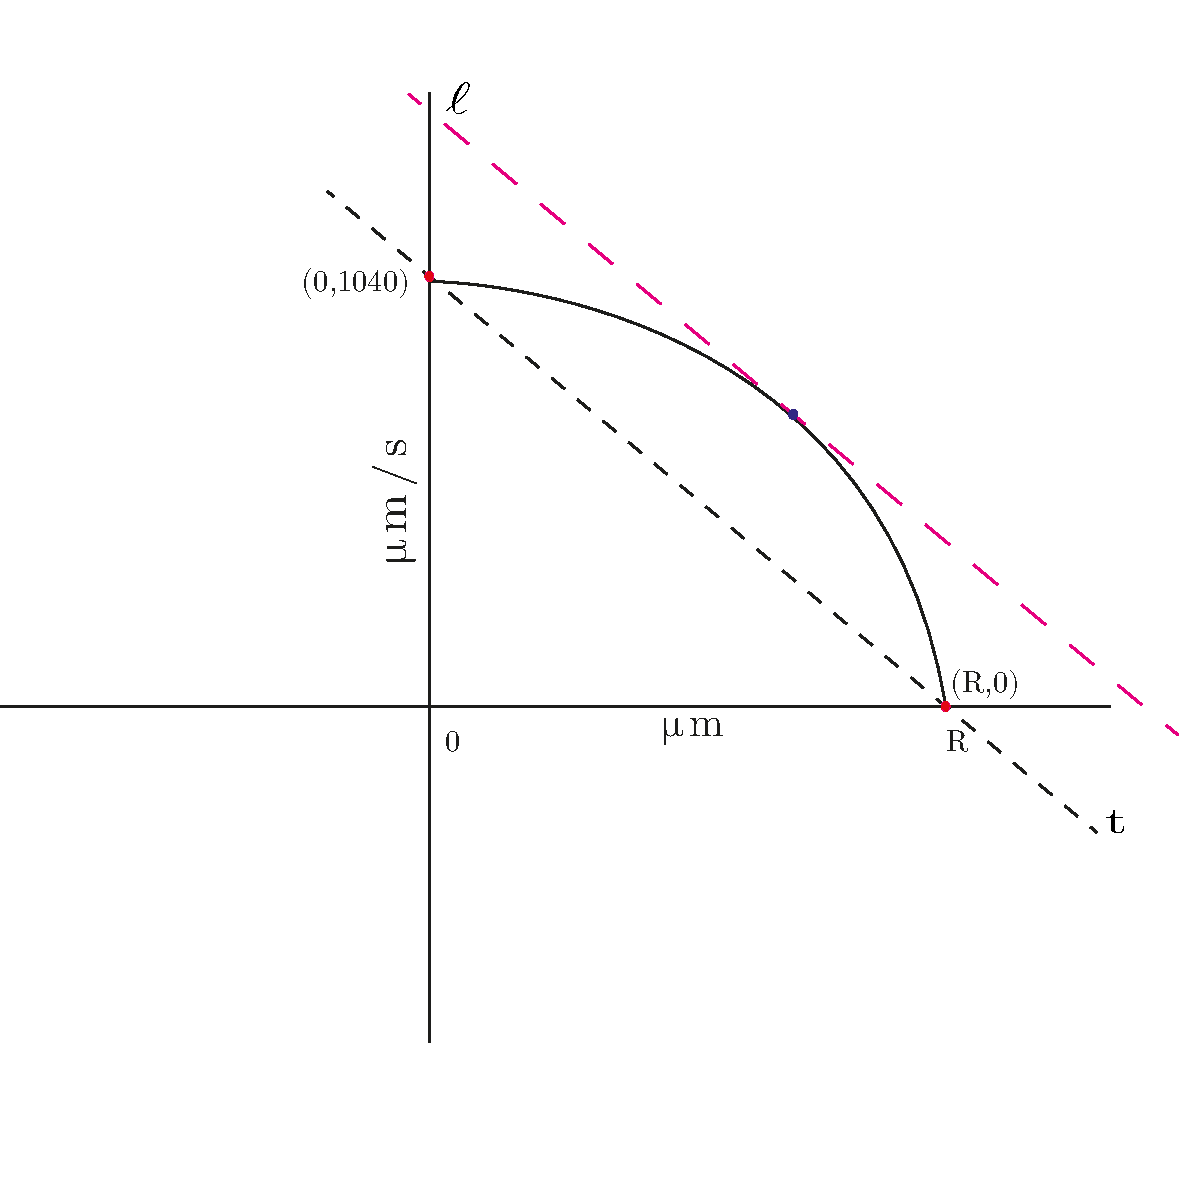
\includegraphics[width=0.50\textwidth]{capitulos/graficas/valmel.pdf}\label{fig:graphic_TVM}
\end{wrapfigure}
Geométricamente toma un significado simple e intuitivo, note la recta que une los puntos (0,1040), (R,0), el teorema de valor medio afirma que existe algún $r$ perteneciente a (0,R) (tal como habíamos mencionado antes) que bajo la imagen de $v^{'}$ es exactamente a la tasa de variación media de $v$ en [a,b], o sea, existe alguna recta $l$ paralela a la recta $t$ dentro del intervalo (0,R).
Nuestro objetivo será encontrar ese punto $r$ en (0,R) que bajo $v^{'}$ sea igual a la T.V.M de $v$ en [0,R], para esto tendremos que recordar la derivada de $v$ (\ref{derivative_one}), véase a continuación.
\begin{align*}
    v^{'}(r)=-\frac{Pr}{2\eta l}. \hspace{0.1cm}\label{derivative_one} \text{ ($Note\ que \ es \ lineal \ en\ v)$ }
\end{align*}
Además
\begin{align*}
    T.V.M[0,R]=-\dfrac{PR}{4l\eta}.
\end{align*}
Entonces debemos buscar un $r$ que satisfaga
\begin{align*}
    v^{'}(r)&=-\frac{Pr}{2\eta l},
\end{align*}
o sea, que
\begin{align*}
    -\frac{Pr}{2\eta l}&=-\dfrac{PR}{4l\eta}
\end{align*}
y, resolviendo la ecuación para $r$
\begin{align*}
     -\frac{Pr}{2\eta l}&=-\dfrac{PR}{4l\eta}\\
      r&=\dfrac{PR\cdot\left(2\eta l\right)}{4Pl\eta}\\
      r&=\frac{R}{2}.
\end{align*}\\
Asignando el valor de R que acordamos en la sección referente a la primera y segunda derivada tenemos que el $r$ que satisface la expresión anterior es: 40 [$\mu m$], es interesante ver que precisamente el $r$ que satisface esto es la mitad del radio de una arteria de radio $R$ (lo cual es simple, pero no es muy trivial de deducir), más aún, $(40,780)$ es el punto de $v$ tal que si trazamos una recta tangente $l$ se puede demostrar que es paralela con la recta $t$ (ya que su pendiente es la misma $\blacksquare$), véase en la figura \ref{fig:graphic_TVM}. Ver estos resultados hace que la tarea de analizar funciones que describen algún fenómeno físico, o no, termine siendo todo un viaje lleno de sorpresas de las cuales podamos aprender muchas lecciones en el camino.

Pensar en una interpretación del teorema de valor medio en nuestro contexto de aplicación es un buen ejercicio, y es posible que un valor numérico podría ayudarnos a comprender alguna interpretación de este hecho, calcularemos la T.V.M de $v$ en [0,R] con los valores numéricos usados en la sección I.2.2, obsérvese a continuación:
\begin{align*}
    T.V.M[0,R]&=-\dfrac{PR}{4l\eta}=-\frac{\left(3.9 \cdot 10^{-12}\left[\frac{N}{\mu m^2}\right]\right)\cdot\left(80\left[\mu m\right]\right)}{4\left(2000\left[\mu m\right]\right)\cdot\left(3\cdot10^{-15}\left[\frac{Ns}{\mu m^2}\right]\right)},\\
    T.V.M[0,R]&=-13\ [(\mu m/s)/\mu m].
\end{align*}
Más aún
\begin{align*}
    v'(40)&=-\frac{\left(3.9 \cdot 10^{-12}\left[\frac{N}{\mu m^2}\right]\right)\cdot\left(40 [\mu m]\right)}{2\left(3\cdot10^{-15}\left[\frac{Ns}{\mu m^2}\right]\right)\cdot\left(2000\left[\mu m\right]\right)},\\
    v'(40)&=-13\ [(\mu m/s)/\mu m].\\
\end{align*}
En efecto, la velocidad disminuye -13 ($\mu$m/s) por cada micrómetro que se aleja del eje principal (ver figura \ref{fig:my_label}), pero algo más impactante es que en algún instante preciso la velocidad disminuía a 13 metros sobre segundo por cada metro que se aleja de dicho eje. Realmente resulta interesante el hecho de que la velocidad del flujo sanguíneo en una arteria de radio $R$ decrezca a una velocidad $v$ por cada micrómetro que se aleja del eje mencionado anteriormente, y además que en algún instante de tiempo exacto se haya alejado del eje principal a la misma velocidad.
\\

¡Es impresionante todo lo que podemos decir de alguna función conociendo información sobre su derivada! Analizar una función de manera introspectiva resulta un ejercicio divertido (hasta cierto punto), además que el conocer los puntos finos sobre una función es importante para comprender fenómenos cotidianos que pueden ser descritos en términos de funciones, entender la esencia del significado de la derivada va más allá de derivar e igualar a cero de forma mecanizada, es entender la interpretación en un contexto de interés, esto con el propósito de obtener información impactante sobre lo que significa la función para la persona interesada en comprender lo que modela dicha función; si bien la función puede que no tenga una interpretación ``cotidiana'', no obstante la intención de abstraer datos sobre alguna función persiste en el objetivo del analista, por algún fin que únicamente conoce el interesado o un grupo de interesados. 
\\
\clearpage
\section{Método de Newton-Raphson}
Sin lugar a duda el método de Newton-Raphson ha sido uno de los más populares para encontrar raíces de funciones (de variable real) no triviales, algo interesante de este algoritmo es que en ocasiones puede funcionar bastante bien, no obstante si nos alejamos mínimamente de un valor óptimo de la condición inicial, puede llegar a fallar, aunado a ello resulta todo un arte encontrar un valor inicial adecuado. En nuestro caso, la función $v$ que es de nuestro interés resulta ``trivial'', el problema únicamente se reduce a solucionar la ecuación cuadrática para algún radio $r$ que satisfaga $$  0=\frac{P}{4\eta l}(R^{2}-r^{2}), $$ si resolvemos la ecuación para $r$ obtenemos que $r_{1}=80[\mu m] \ \& \ r_{2}=-80[\mu m]; $ tomaremos la solución positiva, ya que es evidente que por nuestros propósitos (y para otros) es ilógico tomar un radio negativo, mas aún cuando establecimos que $r \in [0,R]$.\\

En esencia, el método de Newton-Raphson es un algoritmo iterativo el cual nos permite encontrar las raíces de una función ``complicada'' (véase la figura \ref{fig:graphic_NEWTO}), por así decirlo; como mencionamos antes, este algoritmo no garantiza que siempre funcione, frecuentemente el método funciona cuando se proporciona un valor para $x_{0}$ cercano a la raíz de una función $f$, un factor importante a parte del mencionado anteriormente, es la naturalidad de la función de la cual deseamos saber sus raíces. Como es sabido, no todas las funciones tienen las mismas características, de ser así, en mi opinión, las funciones serían aburridas, y no existiría motivación alguna para estudiarlas, los matemáticos estarían muy tristes por este hecho (si fuera así). Las posibles características que nos pueden decir si una función se comportará sin ``anomalias'' son: que no tenga múltiples puntos de inflexión ni pendientes muy grandes cerca de la raíz que estamos buscando, esto hará que el algoritmo funcione lo mejor posible.
\subsubsection{Definición del método de Newton-Raphson}
\fbox{\centering\fbox{\parbox{5.5in}{\centering
\vspace{0.2cm}
        \textit{Sea $f:\ [a,b] \mapsto \mathbb{R}$, con f derivable y definida en $[a,b]$, sea $x_{0},$ definimos $\forall n \in \mathbb{N}$}\\
        $x_{n+1}=x_{n}-\cfrac{f(x_{n})}{f^{'}(x_n)}$
        \vspace{0.2cm}.\\
        }}}

\vspace{0.5cm}
Podemos pensar en algún modo de volver nuestra función aún más interesante, para luego aplicar el método de N-R; esto se puede conseguir mediante la \textbf{composición de la función logaritmo natural con la función \textit{v}}; veremos más adelante que las raíces son bastante aproximadas, lo cual resulta aún más interesante, este hecho habla implícitamente sobre la función logaritmo y sus propiedades tan interesantes. Comencemos por mencionar nuestras funciones de interés, les daremos una definición apropiada para aplicar este método, pero antes cambiaremos ``$r$'' por ``$x$'', lo cual no debería suponer algún problema para el lector; únicamente se hace referencia a algún $x$ del eje $X$.
\begin{align*}
    \textit{Sea f}: \mathbb{R^{+}} \mapsto \mathbb{R},\ \ v: [0,R]\mapsto \mathbb{R}\ \ \& \ \ g: [0,R] \mapsto \mathbb{R},\\
    \text{Donde}: \ f(x)=ln(x),\ v(x)=\frac{P}{4\eta l}(R^{2}-x^{2})\ \& \ g(x)=ln(v(x)),
\end{align*}
$g(x)$ es
\begin{align*}
    g(x)=ln\left(\frac{P}{4\eta l}(R^{2}-x^{2})\right).
\end{align*}
rrr
% Lado derecho del paper
\begin{wrapfigure}{r}{0.54\textwidth}
\centering
\begin{tabular}{|| p{2cm} | p{2cm} | p{2cm} ||}
    \hline
    \multicolumn{3}{|c|}{Tabla de datos}\\
    \hline
    \hline
    $n$ & $x_n$ & $g(x_n)$ \\
    \hline
    1 & 79.99650945 &-2.39962258  \\
    \hline
    2 & 79.98813328 & -1.17599512 \\
    \hline
    3 & 79.97417704 & -0.39855618 \\
    \hline
    4 & 79.96398348 & -0.06313411 \\
    \hline
    5 & 79.96388348 & -0.00191370 \\
    \hline
    6 & 79.96152928 & -0.00000182 \\
    \hline
    7 & 79.96152921 & 0 \\
    \hline
    \hline
\end{tabular}
\caption{Aproximación numérica de la raíz de $g.$}
\label{DFA_table}
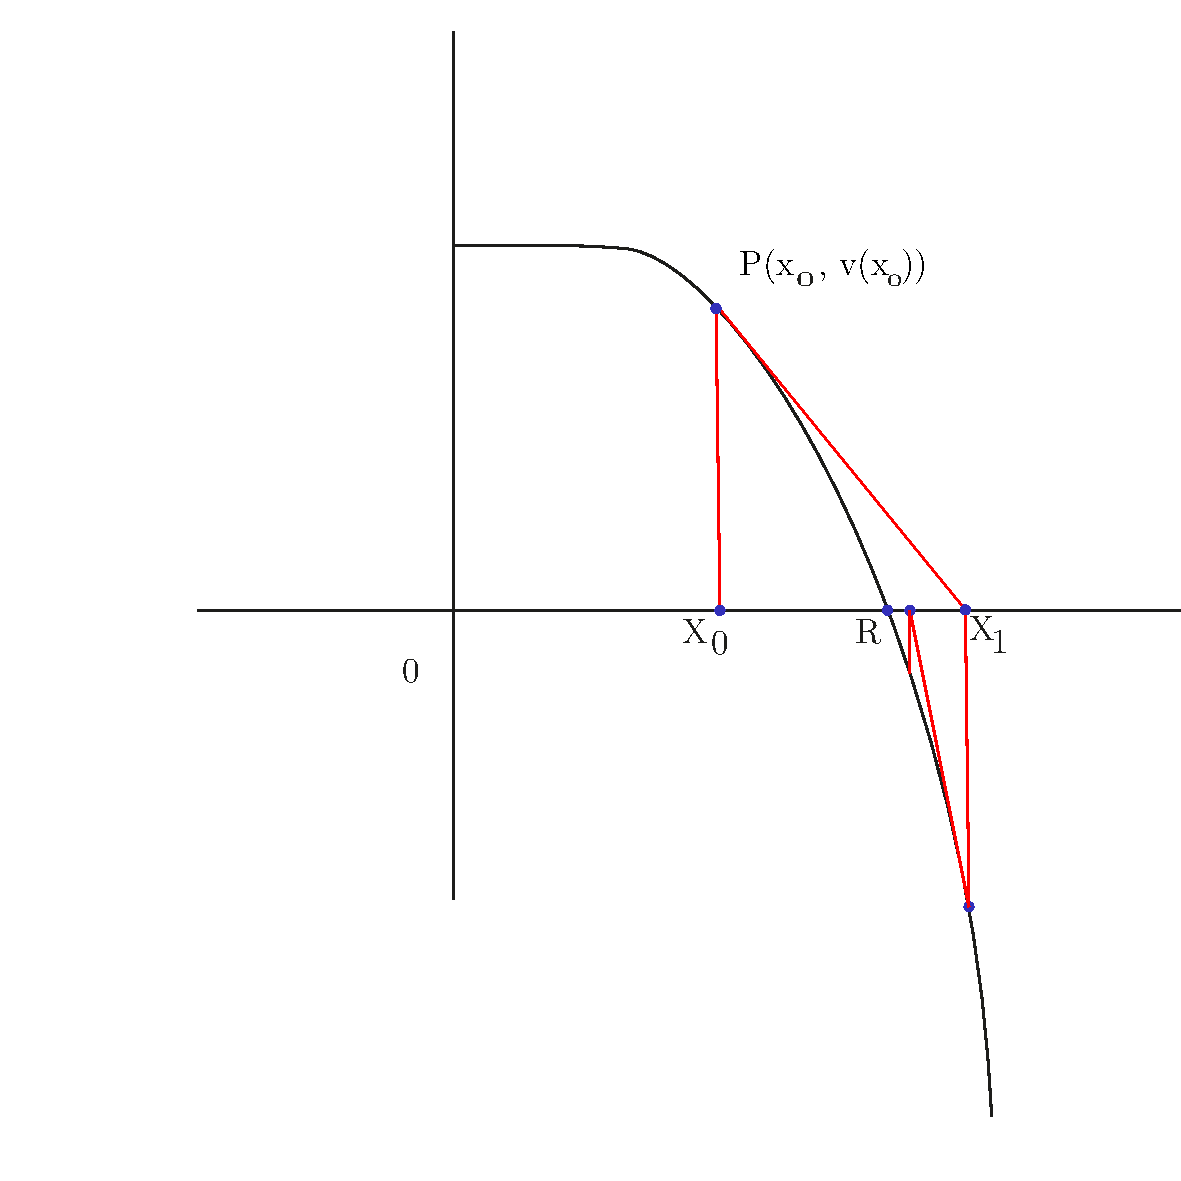
\includegraphics[width=0.45\textwidth]{capitulos/graficas/newto.pdf}\label{fig:graphic_NEWTO}
\end{wrapfigure}

Una vez que conocemos nuestra función de interés procedemos a la aplicación del método de N-R; no es trivial ver que para nuestra función $ln(v(x))$ el $x_0$ tiene que ser exageradamente cercano a la raíz para que el algoritmo no falle, de no ser por la gráfica de la función fallaríamos en el intento de dar un buen $x_0$, y, por consiguiente, sería casi imposible hallar el $x$ donde $ln(v(x))=0$.\\
Dado que conocemos la gráfica de la función (figura \ref{fig:graphic_NEWTO}), y podemos pensar en una idea intuitiva de qué $x_0$ no haría fallar el algoritmo, por ello se motiva a dar un $x_0=79.899$, vea que al disminuir una centésima falla el algoritmo, ¡impresionante!, ¿no es así? Es por ello lo que se comentaba al inicio de la sección, una ligera variación en la condición inicial y el algoritmo podría fallar debido a la naturaleza de la función; particularmente la función $ln(v(r))$ posee la principal característica de tener una pendiente muy grande cerca de la raíz, lo cual provoca que para valores $x_0$ lejanos de dicha raíz el algoritmo falle abruptamente.

Sin embargo para el valor $x_0=79.899$ el algoritmo no presenta ninguna falla, es hasta la séptima iteración donde ya se obtiene la raíz del polinomio (converge rápidamente al valor de la raíz). En la tabla \ref{DFA_table} pueden observarse todos los valores obtenidos durante la ejecución del método; en la primera columna se encuentran los valores que toma $n$, en la segunda los valores de $x_n$ y en la tercera columna su ubican los valores de $f(x_n)$, esta última es importante, nos mostrará qué $x_n$ bajo la imagen de $g$
hace que $g(x)=0$, en la séptima iteración tenemos finalmente que ese ``$x$'', es $x=79.9615292115$. Es fácil ver que el valor de esta raíz es muy cercana al valor que encontramos anteriormente ($80[\mu m]$) resolviendo la ecuación de segundo grado de $v$, esto muestra que la efectividad del algoritmo es buena, no obstante tiene defectos bastante peculiares; después de todo el lector deberá reconocer qué métodos son más factibles para obtener las raíces de la función de su interés.
\clearpage
\section{Conclusiones}
Por el objetivo de este proyecto de aplicación resultó pertinente estudiar todo lo que se pudo sobre
la función $v$ del flujo laminar; el recorrido que hemos hecho a través de las secciones correspondientes
al razonamiento de la función del flujo laminar ha sido, de cierto modo, un poco laborioso fuera del
trabajo de calcular valores numéricos, sino que ha sido así por saber interpretar correctamente lo que
se plantea, de otro modo nos hubiese conducido a un razonamiento erróneo, del cual no tendría ningún
sentido debatir, incluso no tendría nada de sentido tratar de comprenderlo o estudiarlo a profundidad.
No siempre es tan trivial interpretar correctamente las aplicaciones de ciertos teoremas sobre alguna
función de interés, eventualmente uno tiene que respaldarse sobre números, o bien guiarnos sobre algún
sistema de unidades, esto para que tengamos un panorama más claro, sin confusiones cautivadoras a
nublarnos la mirada al momento de analizar una función.

Las interpretaciones que pudimos deducir son muy valiosas, especialmente porque nuestro campo de aplicación es la medicina (¡salvamos vidas!), nuestro análisis contribuye a lograr una comprensión totalitaria de lo que es el flujo sanguíneo, de su comportamiento cuando ciertos parámetros varían, de la velocidad máxima que puede tener el flujo sanguíneo en una artería de radio $R$, y componentes $\eta, \ l, \ P,\ y \ r$; además dedujimos los valores de $r$ para que la velocidad del flujo sanguíneo sea nula, llegamos a dicha interpretación la cual menciona que $r$ debe ser igual al radio de la arteria $R$ para que la velocidad disminuya hasta ser cero por la fricción de las paredes de la arteria; aunado a ello estudiamos el método de Newton-Raphson, el cual nos ayudó a comprender cómo es que podemos hallar las raíces de nuestra función de interés. Si al lector no le parece impresionante todo lo que logramos gracias al cálculo diferencial, no sé que otra cosa lo podría impresionar tanto como comprender una temática abstracta que es natural de los seres vivos...
\chapter{Problemas a resolver}
Ejercicios propuestos al lector obtenidos del libro: \textit{Trascendentes tempranas, de James Stewart.}
\begin{itemize}
 \item Cuando la sangre fluye por un vaso sanguíneo, el flujo F (el
volumen de sangre por unidad de tiempo que corre por un
punto dado) es proporcional a la cuarta potencia del radio R de
ese vaso:
$$F=kR^4.$$
Una arteria parcialmente
obstruida puede expandirse por medio de una operación
llamada angioplastia, en la cual un catéter provisto de un
globo en la punta se infla dentro del vaso a fin de ensancharlo
y restituir el flujo sanguíneo normal.
 Demuestre que el cambio relativo en F es alrededor de cuatro
veces el cambio relativo en R. ¿Cómo afectará un aumento de
5 \% en el radio al flujo de sangre? (Stewart, 2016, p. 256).
\item
Use la ley de Poiseuille para calcular la razón del flujo sanguíneo
en una pequeña arteria humana donde puede tomarse
 $\eta=0.027,\ R=0.008 cm,\ l=2cm\ y\ P=4000\ \tfrac{dinas}{cm^2}$\\ (Stewart, 2016, p. 597).
 \item
 La presión sanguínea alta resulta de la obstrucción de las
arterias. Para mantener un flujo normal, el corazón tiene que
bombear más fuerte, de modo que se incrementa la presión
arterial. Use la ley de Poiseuille para demostrar que si $R_0$ y $P_0$
son valores normales del radio y la presión en una arteria, y
los valores obstruidos son R y P, respectivamente, entonces
para que el flujo permanezca constante, P y R se relacionan
mediante la ecuación

\begin{align*}
    \frac{P}{P_0}=\left(\frac{R_0}{R}\right)^4
\end{align*}
Deduzca que si el radio de una arteria se reduce a tres cuartos
de su valor anterior, entonces la presión es más que el triple (Stewart, 2016, p. 567).

Como observación al ejercicio anterior, opino que sería complementario que el lector experimente con la expresión matemática del ejercicio, es decir, que se cuestione sobre qué pasaría si el radio disminuye 2/5, en vez de 3/4 del valor anterior, además de que investigue por su propia cuenta casos clínicos donde cierto valor de reducción del radio de la arteria (relacionado a una patología) resulta mortal en algún paciente, y cómo es que se puede evitar.
\end{itemize} 
\include{capitulos/Bibliografía}
\end{document}
